
\begin{figure*}[t]
    \centering
    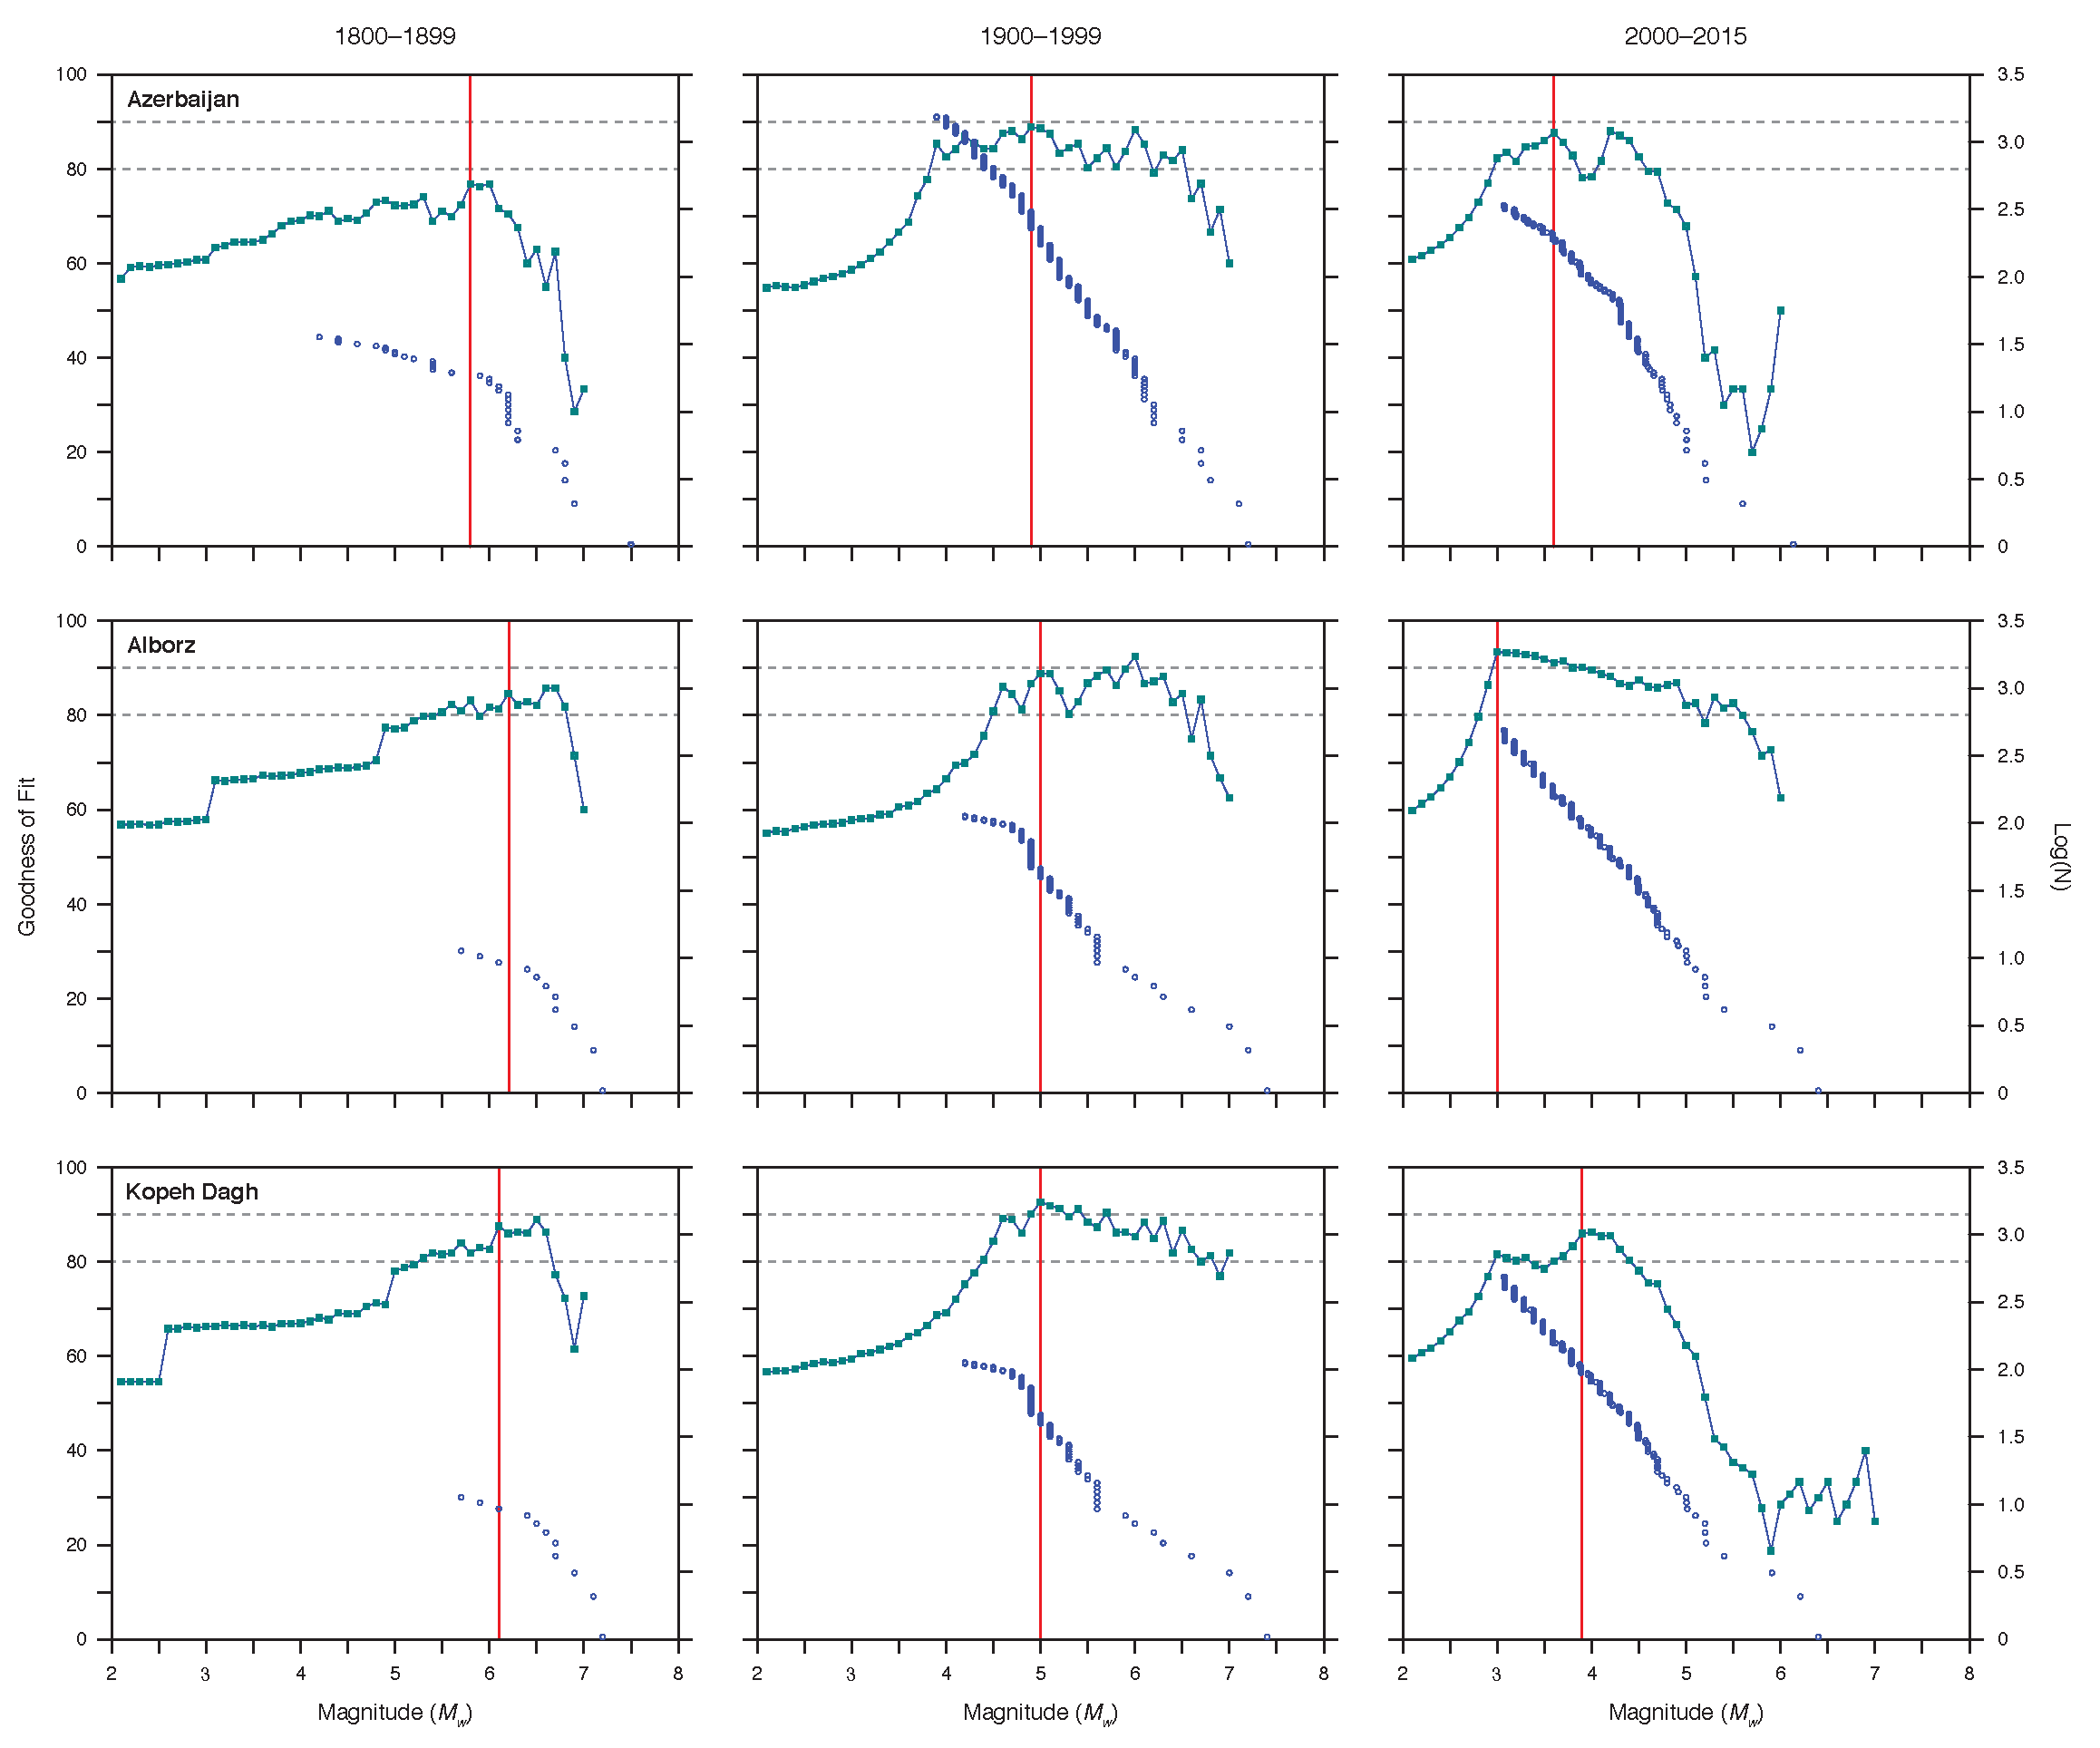
\includegraphics[width=\textwidth]{figures/pdf/figure-06} 
    \caption{Annual probability of exceedance as a function of earthquake magnitude for the seismic zones in the region of interest. The three curves in red correspond to those seismic zones completely considered within the study area, whereas the ones in blue are the two additional contributing zones from the rest of the country. THe last curve in green corresponds to the complete region of interest, here referred to as the uniform model. The shaded range indicates the models' $\pm 1$ standard deviation.}
    \label{fig:annualp}
\end{figure*}

\begin{table}[t]
    \centering
    \caption{Seismicity parameters $b$ and $M_{\max}$ computed for the seismic zones in our region of interest and the reference uniform seismicity model along with the observed maximum magnitude, $M_{\max}^{\mathrm{obs}}$.}
    \begin{tabular}{@{\hspace{0.2ex}}lccc@{\hspace{0.2ex}}}
        \cline{2-4}                                                                         \\[-1.6ex]
                        & $b$-value         & $M_{\max}$        & $M_{\max}^{\mathrm{obs}}$ \\[0.6ex]
        \hline                                                                              \\[-1.6ex]
        Azerbaijan      & 1.10 $\pm$ 0.03   & 7.93 $\pm$ 0.34   & 7.7                       \\
        Alborz          & 1.03 $\pm$ 0.03   & 7.85 $\pm$ 0.66   & 7.8                       \\
        Kopeh Dagh      & 0.89 $\pm$ 0.04   & 7.78 $\pm$ 0.31   & 7.6                       \\
        Zagros          & 0.99 $\pm$ 0.02   & 7.47 $\pm$ 0.26   & 7.4                       \\
        Central-East    & 0.95 $\pm$ 0.04   & 7.84 $\pm$ 0.34   & 7.6                       \\
        Uniform Model   & 0.90 $\pm$ 0.02   & 7.87 $\pm$ 0.26   & 7.8                       \\[0.5ex]
        \hline 
    \end{tabular}
    \label{tab:params} 
\end{table}

\section{Seismicity Parameters}

Following the general approach described in the previous sections and using the information collected about the seismic catalog and its completeness, we computed the seismicity parameters $a$ and $b$, and the maximum magnitude $M_{\max}$ using the seismic hazard assessment software HA3 (version 3). This software implements the procedures developed by \citet{Kijko_1989_BSSA, Kijko_1992_BSSA}, and subsequent updates by \citet{Kijko_2004_PAG}. HA3 is widely used for this type of computations and is regarded as a reliable tool in seismic hazard analysis \citep[see, for instance,][]{Karimiparidari2013, Khodaverdian_2016_BSSA}.

The $a$-value is estimated based on the completeness year, the correlation distance, and the number of events per grid cell. We assume magnitude increments of $\Delta M = 0.1$, count events with magnitude $M_w > 3$, and smooth the number of events for each cell. This means each cell has a different $a$-value and thus the result is variable throughout our region of interest. On the other hand, we consider the $b$-value and $M_{\max}$ to be constant within each of the seismic zones in our study area. We compute $b$ and $M_{\max}$ using HA3 and the information from the catalog, which we divide in four sub-catalogs: 2 incomplete catalogs for the prehistorical (before 1000) and historical (between 1000 and 1799) events, and two complete catalogs for pre-instrumental (between 1800 and 1899) and instrumental (between 1900 and 2015) events. In this process we use the values of $M_c$ shown in Table \ref{tab:completeness}. In a recent hazard analysis for whole Iran, \citet{} used variable values of $M_c$ for individual sub-catalogs. This is an additional level of complexity we may consider in the future. 

We obtain $b$ and $M_{\max}$ for two different models. In the first model we obtain these parameters independently for each one of the five seismic zones influencing the hazard in northern Iran. That is, we obtain distinct values of $b$ and $M_{\max}$ for the main northern seismic zones of Azerbaijan, Alborz, and Kopeh Dagh, as well as for the portions of the Zagros and Central-East seismic zones contributing to our region of interest (see Fig.~\ref{fig:iran} for reference). In the second model we consider the whole study area as a uniform seismic zone. Admittedly, this assumption is unrealistic if considered from the point of view that different seismic zones have different seismicity parameters. Computing results for this uniform model is, nonetheless, useful for the analysis of results and comparisons with other studies. Table \ref{tab:params} shows the parameters $b$ and $M_{\max}$ obtained with HA3 for the five seismic zones and the uniform regional model, along with the observed maximum magnitude, $M_{\max}^{\mathrm{obs}}$; and Fig.~\ref{fig:annualp} shows the annual probability of exceedance as a function of earthquake magnitude.

% *********************************************************************************************************************
% OLD
% *********************************************************************************************************************

% For each of the three seismic regions, Gutenberg-Richter parameters and maximum magnitude ($M_{max}$) were calculated using Seismic Hazard Assessment code (HA3) \citep{kijko2004}. The regional maximum magnitude for each region is estimated by the \citet{Kijko1989} method, which is implemented in the HA3 package. For smoothed seismicity areas, $b-value$ is assumed constant. The $a-value$ can vary spatially and is determined by counting earthquakes above $M$ 3.0 in each grid cells.

% \citet{Karimiparidari2013} applied the Maximum Curvature (MAXC) technique \citep{Wyss1999, Wiemer2000} by ZMap \citep{Wiemer2001} to calculate the level of completeness of instrumental part of the catalog.  Following the \citet{Karimiparidari2013}, we assume the catalog is complete for earthquakes with magnitude 4.5, 4.4, 4.5, 4.5, and 4.4 for Azerbaijan, Alborz,  Kopeh-Dagh, Central Iran, and Zagros tectonic seismic regions, respectively. For the uniform model we used 4.5 as a completeness magnitude. In this study we use those magnitudes of completeness as the magnitude threshold in the calculation of the seismicity parameters. We also used the seismicity parameters of \citet{Karimiparidari2013} as the priory information in HA3 code. The updated values are displayed in Table \ref{tab:b_value}.  Annual occurrence rate of the earthquake for each region is shown in Fig.~\ref{fig:annual_m}.

% *********************************************************************************************************************
% OLDER
% *********************************************************************************************************************

% For each of the three seismic regions, Gutenberg-Richter parameters and Max magnitude ($M_{max}$) were calculated using Seismic Hazard Assessment code (HA3) \citep{kijko2004}. The regional maximum magnitude for each region is estimated by the \citet{Kijko1989} method, which is implemented in the HA3 package. For smoothed seismicity areas, $b-value$ is assumed constant. The $a-value$ can vary spatially and is determined by counting earthquakes above $M$ 3.0 in grid cells.\\

% \citet{Karimiparidari2013} applied the Maximum Curvature (MAXC) technique \citep{Wyss1999, Wiemer2000} by ZMap \citep{Wiemer2001} to calculate the level of completeness of instrumental part of the catalog. In this study we use those magnitudes of completeness as the magnitude threshold in the calculation of the seismicity parameters. We also used the seismicity parameters of this study \citep{Karimiparidari2013} as the priory information in HA3 code. The updated values are displayed in Table 2.

% Following the \citet{Karimiparidari2013}, we assume the catalog is complete for earthquakes with magnitude 4.5, 4.4, and 4.5 for Azerbaijan, Alborz and Kopeh-Dagh tectonic seismic regions, respectively. The completeness of each region can be seen easily from the scatter plot of completeness test. 
